\documentclass[conference]{IEEEtran}
\IEEEoverridecommandlockouts
% The preceding line is only needed to identify funding in the first footnote. If that is unneeded, please comment it out.
\usepackage{cite}
\usepackage{amsmath,amssymb,amsfonts}
\usepackage{graphicx}
\usepackage{textcomp}
\usepackage{xcolor}

\usepackage{subcaption}

\usepackage[draft,hidelinks,bookmarks=false,bookmarksdepth=0]{hyperref}
\usepackage{xurl}  


\usepackage{listings}

\def\BibTeX{{\rm B\kern-.05em{\sc i\kern-.025em b}\kern-.08em
    T\kern-.1667em\lower.7ex\hbox{E}\kern-.125emX}}
\begin{document}

\title{Carbon Footprint of Document-oriented and Relational Storage for Image-based Time-Series Workloads}

\author{
[Hidden for double-blind review]
}


\maketitle

\begin{abstract}
Smart building and facility-monitoring systems increasingly deploy IoT cameras that store high-resolution images inline in time-series databases. Selecting the right storage backend affects not only performance but also energy consumption and carbon emissions---a critical concern for green building initiatives. This paper measures and compares the carbon footprint of PostgreSQL (TimescaleDB) and MongoDB for image-based time-series workloads across four resolutions: 1080p ($\sim$1.09~MB), 1440p ($\sim$1.66~MB), 4K ($\sim$3.07~MB), and 5K ($\sim$4.83~MB). Using isolated Dockerized deployments and CodeCarbon energy tracking, we find that the complete MongoDB benchmark phase consumes 0.00157~kWh and emits 1064~mg CO$_2$eq---\textbf{20.3\% more} than PostgreSQL's 0.00131~kWh and 884~mg CO$_2$eq. The gap widens with resolution: estimated per-resolution emissions diverge sharply above 1440p as MongoDB's WiredTiger cache eviction and BSON serialization overhead grow with payload size. PostgreSQL's TOAST mechanism isolates large binary payloads out-of-line, maintaining stable $1.04\times$ storage amplification versus MongoDB's $2.99\times$ at 4K. These findings provide resolution-dependent guidance for carbon-aware database selection in green IoT deployments.
\end{abstract}

\begin{IEEEkeywords}
time-series databases, IoT building monitoring, PostgreSQL, MongoDB, carbon footprint, green computing, inline image storage
\end{IEEEkeywords}

\section{Introduction}
\label{sec:introduction}

Modern smart building and facility-monitoring systems deploy dense networks of IoT cameras and environmental sensors to support occupancy analysis, safety auditing, and predictive maintenance~\cite{bajera_iot_smart_buildings,alfuqaha_iot_survey}. These devices continuously capture high-resolution images---from 1080p security feeds to 4K inspection cameras---which must be stored inline alongside timestamped metadata for temporal queries and audit replay~\cite{ceec_tsdb_review,jensen_tsms_survey}. As green building standards increasingly account for the operational carbon cost of IT infrastructure~\cite{nerc_tsdb_survey}, the choice of storage backend is no longer purely a performance decision: it directly affects the energy consumed by the data tier running 24/7 at the edge or in an on-premises data center.

Organizations commonly reuse existing general-purpose databases for this role. PostgreSQL~\cite{postgresql_official} with TimescaleDB~\cite{timescaledb_official} extends a proven relational engine with hypertable chunking and employs TOAST~\cite{postgresql_toast_docs} to relocate large binary payloads out-of-line. MongoDB~\cite{mongodb_official} offers native Time-Series Collections backed by the WiredTiger~\cite{mongodb_wiredtiger_storage} storage engine with Snappy~\cite{google_snappy} block compression, storing entire BSON documents---including multi-megabyte image binaries---inline in B-Tree pages~\cite{timescale_mongodb_comparison}. This inline vs.\ out-of-line architectural difference is expected to produce divergent energy profiles as image resolution grows.

Existing benchmarks~\cite{tsbs,cratedb_ts_benchmark,diva_timescaledb_mongodb_eval} target lightweight numeric payloads and do not measure energy or emissions. No study evaluates the carbon cost of storing multi-megabyte image frames across varying resolutions in containerized environments.

\textbf{Research Question:} \textit{What is the carbon footprint of inline image-based time-series storage in PostgreSQL (TimescaleDB) versus MongoDB across varying camera resolutions, and which engine is more energy-efficient for IoT building monitoring?}

We benchmark both engines across four resolutions (1080p--5K) using Docker containers, measure end-to-end CO$_2$ emissions with CodeCarbon~\cite{codecarbon}, and report supporting performance metrics to explain the observed energy differences.

\section{Related Work}
\label{sec:related_work}

Time-series databases optimize sequential data ingestion by employing append-only storage, time-based partitioning, and columnar compression to bypass the write amplification inherent in traditional B-Tree indexes~\cite{dewaal_timeseries_survey,jensen_tsms_survey}. TimescaleDB~\cite{timescaledb_official} extends PostgreSQL~\cite{postgresql_official} with transparent hypertable chunking that sustains flat ingestion throughput at scale~\cite{dewaal_timeseries_survey,nerc_tsdb_survey}. MongoDB~\cite{mongodb_official} introduced native Time-Series Collections in version 5.0, which internally bucket measurements into compacted documents optimized for columnar access patterns~\cite{timescale_mongodb_bad_idea,mongodb_ts_best_practices}.

Existing comparative benchmarks between these systems are limited to lightweight scalar payloads. The TSBS suite~\cite{tsbs} generates synthetic JSON/SQL events of a few bytes each. The evaluation by Mohamud and Broström~\cite{diva_timescaledb_mongodb_eval} compared TimescaleDB and MongoDB query execution times using numerical sensor data. CrateDB's benchmark~\cite{cratedb_ts_benchmark} focused on aggregate throughput over numeric IoT metrics. These studies typically do not incorporate binary payloads exceeding a few kilobytes.

This gap is significant because storage engine behavior changes fundamentally with payload size. MongoDB's WiredTiger~\cite{mongodb_wiredtiger_storage} uses Snappy~\cite{google_snappy} block compression that achieves excellent ratios on repetitive JSON structures but offers negligible compression on high-entropy binary data such as JPEG images. PostgreSQL's TOAST~\cite{postgresql_toast_docs} mechanism stores oversized attributes out-of-line in a separate table, an approach specifically designed for large binary values. MongoDB's alternative for large binaries---GridFS~\cite{mongodb_gridfs}---chunks files into 255~KB segments, but is incompatible with native Time-Series Collections~\cite{mongodb_ts_limitations}.

The carbon footprint of computing infrastructure has attracted growing attention. Lannelongue et al.~\cite{lannelongue_green_algorithms} introduced the Green Algorithms framework, quantifying CO$_2$-equivalent emissions from computation using energy consumption and regional grid intensity---the same principle adopted by CodeCarbon~\cite{codecarbon}. Strubell et al.~\cite{strubell_energy_nlp} highlighted the disproportionate energy cost of large-scale model training, catalysing interest in per-operation energy accounting across the software stack. Within the database domain, energy efficiency studies have focused on query optimisation~\cite{nerc_tsdb_survey} and hardware selection, but no prior work applies per-operation carbon accounting to binary time-series storage engines under varying payload sizes.

Our work directly addresses this gap by conducting a systematic multi-resolution benchmark (1080p--5K) for IoT building monitoring, measuring both performance and carbon footprint via CodeCarbon.


\section{Methodology}
\label{sec:methodology}

\subsection{Hardware and Software Environment}
All experiments execute on a single host machine running Linux 6.8.0 with an 11th Gen Intel Core i7-1165G7 processor (4 cores / 8 threads, 2.80~GHz base, 28~W TDP) and 15.3~GB RAM. The machine is located in Indonesia (Java grid region); CodeCarbon uses the corresponding national carbon intensity factor. Containers share host CPU and memory with no explicit CPU pinning or memory limits beyond the MongoDB WiredTiger cache cap. Table~\ref{tab:software_versions} lists the software stack.

\begin{table}[htbp]
\centering
\renewcommand{\arraystretch}{1.1}
\caption{Software Stack}
\label{tab:software_versions}
\begin{tabular}{ll}
\hline
\textbf{Component} & \textbf{Version} \\
\hline
Host OS         & Linux 6.8.0-90-generic (x86\_64) \\
Docker          & Compose v2 \\
PostgreSQL      & 15 + TimescaleDB 2.x \\
MongoDB         & 7.0 \\
Python          & 3.12.3 \\
psycopg2        & (latest) \\
pymongo         & (latest) \\
CodeCarbon      & 3.2.5 \\
\hline
\end{tabular}
\end{table}

\subsection{Environment and Workloads}
All experiments run in isolated Docker~\cite{docker_official} containers: PostgreSQL~15 with TimescaleDB~\cite{timescaledb_official} using default shared buffers, and MongoDB~7.0~\cite{mongodb_official} with \texttt{--wiredTigerCacheSizeGB~2} (a realistic IoT gateway constraint). The 2~GB WiredTiger cache approximates the auto-configured value on an IoT gateway with 4--8~GB RAM and reflects realistic containerised edge deployments. Four quality-100 JPEG resolutions simulate building-camera payloads: 1080p ($1920{\times}1080$, $\sim$1.09~MB), 1440p ($2560{\times}1440$, $\sim$1.66~MB), 4K~UHD ($3840{\times}2160$, $\sim$3.07~MB), and 5K ($5120{\times}2880$, $\sim$4.83~MB). Maximum-quality JPEG ensures high visual entropy that defeats internal compression, reflecting worst-case inline storage.

\subsection{Schema and Operations}
PostgreSQL stores each frame as a \texttt{BYTEA} row in a TimescaleDB hypertable; TOAST~\cite{postgresql_toast_docs} automatically relocates payloads exceeding $\sim$2~KB out-of-line. MongoDB stores functionally equivalent documents with the binary payload as inline \texttt{BinData}~\cite{mongodb_bson_spec} in a native Time-Series Collection (Snappy-compressed WiredTiger B-Tree). Both schemas carry a compound index on \texttt{(device\_id, ts~DESC)}.

For each resolution, 100 records are inserted in batches of 50 (5 runs), followed by 15 binary retrieval runs that fully materialise the \texttt{payload\_data} column for 100 rows. The 5K profile uses a smaller batch size of 25 to avoid exceeding MongoDB's 16~MB per-document BSON limit under worst-case framing. Each engine is wiped and rebuilt between resolutions. Storage amplification is measured as on-disk size divided by raw payload size.

\subsection{Carbon Footprint Measurement}
Each engine phase runs as a single CodeCarbon~\cite{codecarbon}-tracked process. CodeCarbon estimates CPU and RAM power draw and converts total energy to CO$_2$-equivalent using regional grid intensity. All operations for a given engine (insertions and retrievals across all four resolutions) are aggregated into one measurement, isolating per-engine carbon cost under identical hardware conditions. Per-resolution emissions are estimated using a constant power-rate model: the measured total energy $E$ and duration $T$ yield an average power $P = E/T$; each profile's estimated energy is then $P \times t_i$, where $t_i$ is the sum of mean insertion and retrieval times for that profile across all runs. This model assumes constant CPU and RAM power draw, which is a simplification---actual power varies between write-intensive and read-intensive phases---but provides a principled first-order breakdown consistent with CodeCarbon's own TDP-based estimation.

Note that CodeCarbon detected the two engine phases as running in slightly different sub-regions of the same grid (``banten'' and ``jakarta''); both map to the same national Indonesia carbon intensity factor, so emissions comparisons remain valid.


\begin{table}[htbp]
\centering
\renewcommand{\arraystretch}{1.1}
\caption{Insert Throughput, Retrieval Latency, and Storage (100 rows)}
\label{tab:performance_summary}
\begin{tabular}{l r r r r r r}
\hline
\textbf{Res.} & \multicolumn{2}{c}{\textbf{Insert (r/s)}} & \multicolumn{2}{c}{\textbf{Retr. (ms)}} & \multicolumn{2}{c}{\textbf{Storage amp.}} \\
 & \textbf{PG} & \textbf{MG} & \textbf{PG} & \textbf{MG} & \textbf{PG} & \textbf{MG} \\
\hline
1080p & 21.7  & \textbf{113.2} & 687  & \textbf{283}  & 1.04$\times$ & \textbf{0.12$\times$} \\
1440p & 16.6  & \textbf{26.6}  & 1061 & \textbf{478}  & 1.04$\times$ & \textbf{0.77$\times$} \\
4K    & \textbf{9.9}  & 5.5   & 2448 & \textbf{742}  & \textbf{1.04$\times$} & 2.99$\times$ \\
5K    & \textbf{6.7}  & 2.9   & 3916 & \textbf{1406} & \textbf{1.04$\times$} & 3.04$\times$ \\
\hline
\end{tabular}
\end{table}

\begin{table*}[htbp]
\centering
\renewcommand{\arraystretch}{1.1}
\caption{Per-Resolution Carbon Footprint Breakdown (estimated via constant power-rate model). PG = PostgreSQL, MG = MongoDB. Bold = higher cost per row.}
\label{tab:carbon_summary}
\begin{tabular}{l rr rr rr rr rr}
\hline
\textbf{Res.}
  & \multicolumn{2}{c}{\textbf{Duration (s)}}
  & \multicolumn{2}{c}{\textbf{Energy (µWh)}}
  & \multicolumn{2}{c}{\textbf{CPU (µWh)}}
  & \multicolumn{2}{c}{\textbf{RAM (µWh)}}
  & \multicolumn{2}{c}{\textbf{Emissions (mg CO$_2$eq)}} \\
  & PG & MG & PG & MG & PG & MG & PG & MG & PG & MG \\
\hline
1080p & 33.9 & \textbf{9.7}  & \textbf{117.6} & 34.1  & \textbf{26.6} & 8.0   & \textbf{91.0}  & 26.1  & \textbf{79.5}  & 23.1  \\
1440p & 49.2 & \textbf{27.5} & \textbf{170.5} & 96.4  & \textbf{38.6} & 22.6  & \textbf{132.0} & 73.8  & \textbf{115.3} & 65.2  \\
4K    & \textbf{89.4} & 106.4 & 309.8 & \textbf{373.2} & 70.1 & \textbf{87.5} & 239.7 & \textbf{285.7} & 209.4 & \textbf{252.2} \\
5K    & \textbf{134.5} & 191.7 & 466.2 & \textbf{672.3} & 105.5 & \textbf{157.7} & 360.7 & \textbf{514.7} & 315.1 & \textbf{454.5} \\
\hline
\textbf{Total} & 377.5 & \textbf{448.7} & 1310 & \textbf{1574} & 296 & \textbf{369} & 1012 & \textbf{1205} & 884 & \textbf{1064} \\
\hline
\end{tabular}
\end{table*}




\section{Results}
\label{sec:results}

\begin{figure}[t]
\centering

\includegraphics[width=\columnwidth]{figures/boxplot_insert_throughput.pdf}
\caption{Insert throughput (1080p--5K). MongoDB leads at 1080p; PostgreSQL overtakes above 1440p.}
\label{fig:insert_throughput}
\end{figure}

\begin{figure}[t]
\centering

\includegraphics[width=\columnwidth]{figures/boxplot_retrieval_latency.pdf}
\caption{Binary retrieval latency (100 rows, log scale). MongoDB leads at all resolutions (1080p--5K).}
\label{fig:retrieval_latency}
\end{figure}

\begin{figure}[t]
\centering
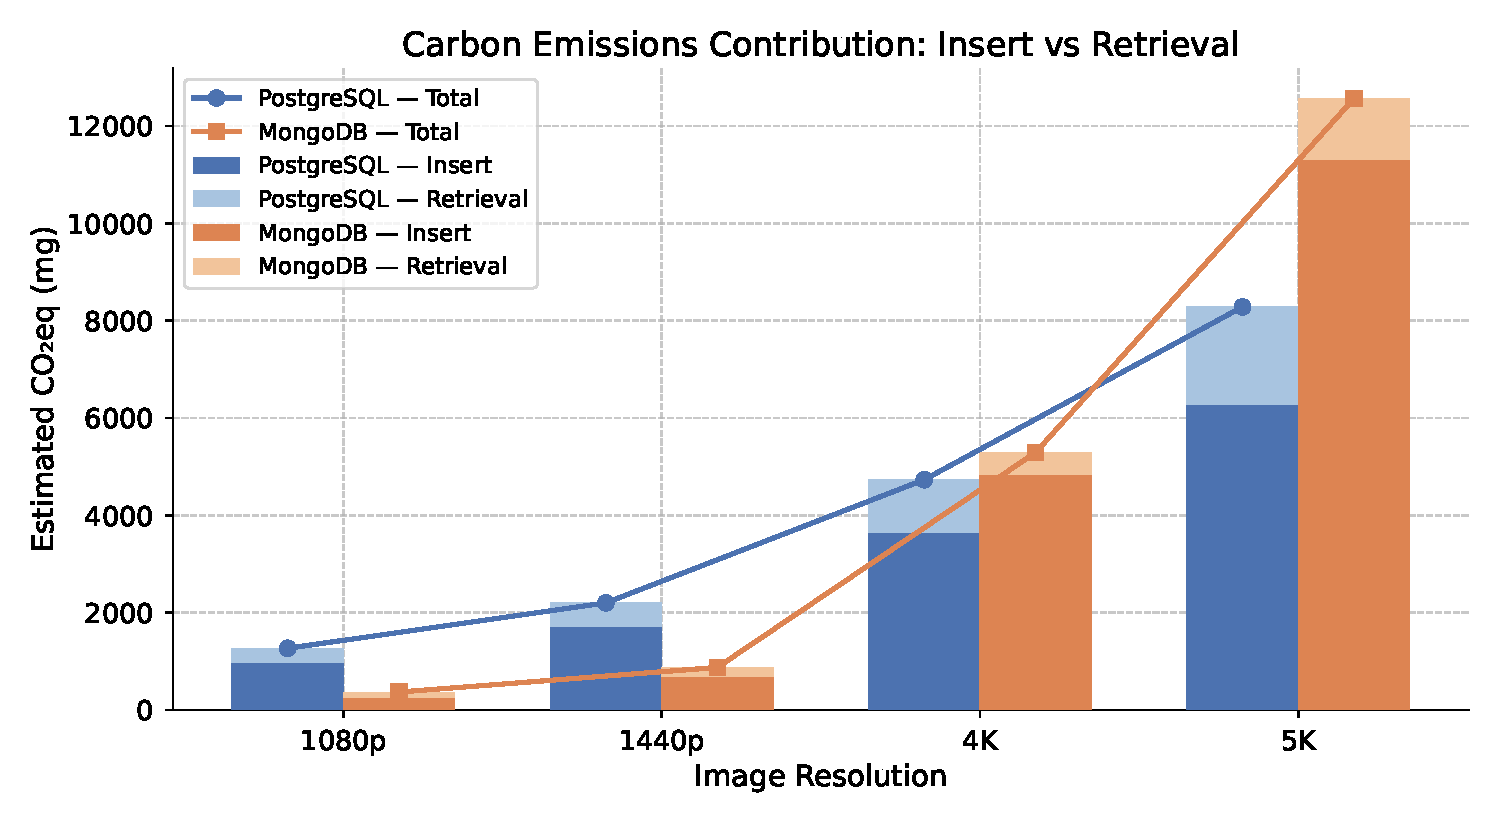
\includegraphics[width=\columnwidth]{figures/carbon_footprint.pdf}
\caption{Estimated CO$_2$ emissions (mg) per resolution. MongoDB diverges sharply from PostgreSQL above 1440p.}
\label{fig:carbon_footprint}
\end{figure}

\begin{figure*}[t]
\centering

\includegraphics[width=\textwidth]{figures/carbon_breakdown.pdf}

\caption{Per-resolution carbon breakdown (estimated via constant power-rate model): benchmark duration, total energy, CPU energy, RAM energy, and CO$_2$ emissions. MongoDB exceeds PostgreSQL above 1440p across all components.}
\label{fig:carbon_breakdown}
\end{figure*}

\subsection{Supporting Performance Observations}
\label{subsec:performance}
Table~\ref{tab:performance_summary} and Figures~\ref{fig:insert_throughput}--\ref{fig:retrieval_latency} summarise the performance results. Insertion throughput crosses over between 1440p and 4K: MongoDB leads at 1080p (113.2 vs.\ 21.7~r/s) and 1440p (26.6 vs.\ 16.6~r/s), but PostgreSQL overtakes at 4K (9.9 vs.\ 5.5~r/s) and 5K (6.7 vs.\ 2.9~r/s). Binary retrieval shows a consistent advantage for MongoDB across \emph{all} resolutions: $2.4\times$ faster at 1080p (283 vs.\ 687~ms), $2.2\times$ at 1440p (478 vs.\ 1061~ms), $3.3\times$ at 4K (742 vs.\ 2448~ms), and $2.8\times$ at 5K (1406 vs.\ 3916~ms). MongoDB's inline \texttt{BinData} storage enables direct sequential reads from contiguous B-Tree leaf pages, avoiding PostgreSQL's TOAST pointer dereference to a secondary table. Storage amplification shows a resolution-dependent regime change for MongoDB: $0.12\times$ at 1080p (Snappy effectively compresses small documents where JSON metadata dominates) rising to $0.77\times$ at 1440p, then exploding to $2.99\times$ at 4K and $3.04\times$ at 5K as the JPEG binary payload begins to dominate document size and defeats block compression.

\subsection{Carbon Footprint (RQ)}
\label{subsec:carbon_footprint}
Table~\ref{tab:carbon_summary} and Figure~\ref{fig:carbon_footprint} report energy and emissions. The complete MongoDB phase consumed 0.00157~kWh over 448.7~s, emitting 1064~mg CO$_2$eq. PostgreSQL consumed 0.00131~kWh over 377.5~s, emitting 884~mg CO$_2$eq---a \textbf{20.3\% carbon advantage for PostgreSQL}. RAM dominates both ($\sim$77\% of total energy); CPU energy is 24.7\% higher for MongoDB. Per-resolution estimates (Figures~\ref{fig:carbon_footprint} and~\ref{fig:carbon_breakdown}) reveal a nuanced picture. At 1080p, MongoDB's faster insertion (113 vs.\ 22~r/s) means it completes the profile $3.5\times$ faster (9.7 vs.\ 33.9~s), so it actually emits \emph{less} per resolution (23 vs.\ 80~mg CO$_2$eq). The same holds at 1440p (65 vs.\ 115~mg). The crossover occurs at 4K, where MongoDB's insertion slows drastically due to WiredTiger cache eviction (5.5 vs.\ 9.9~r/s), causing it to take 19\% longer (106.4 vs.\ 89.4~s) and emit 20\% more (252 vs.\ 209~mg). At 5K the gap widens to 44\% more time and 44\% more emissions for MongoDB (455 vs.\ 315~mg). The aggregate 20.3\% carbon premium for MongoDB therefore reflects the dominance of the high-resolution profiles, which contribute the majority of total benchmark time.


\section{Discussion}
\label{sec:discussion}

\textbf{Why MongoDB costs more energy.} MongoDB's WiredTiger engine stores entire BSON documents---including multi-megabyte \texttt{BinData} image payloads---inline in B-Tree leaf pages~\cite{mongodb_bson_spec,mongodb_wiredtiger_storage}. As payloads grow above $\sim$1.5~MB, the working set no longer fits in the 2~GB WiredTiger cache; eviction threads stall application threads to flush dirty pages~\cite{percona_wiredtiger_eviction}, prolonging execution and elevating CPU/RAM energy. At low resolutions (1080p--1440p), Snappy's block compression is effective because the document is small enough that the structured JSON metadata constitutes a significant compressible fraction, explaining MongoDB's $0.12\times$ amplification at 1080p. However, as payload size grows above $\sim$1.5~MB, the high-entropy JPEG binary dominates the document and defeats block compression~\cite{mongodb_wiredtiger_storage}, causing the $3\times$ storage amplification at 4K--5K and the corresponding extra write I/O energy. GridFS would avoid inline storage but is incompatible with native Time-Series Collections~\cite{mongodb_ts_limitations}.

\textbf{Why PostgreSQL is more efficient.} TOAST~\cite{postgresql_toast_docs} relocates payloads exceeding $\sim$2~KB out-of-line into a sequentially-organised secondary table, leaving only a small pointer in the main hypertable row. This keeps the primary B-Tree compact for fast index traversal regardless of resolution, produces stable $1.04\times$ amplification, and avoids the page-rewrite amplification that stalls WiredTiger. The resulting lower I/O volume and shorter execution time ($-19\%$) directly translate to lower energy consumption. Notably, MongoDB's inline storage \emph{does} deliver faster binary retrieval at all resolutions ($2.2$--$3.3\times$)---a genuine advantage of the document model for read-heavy workloads---but this benefit is outweighed in energy terms by MongoDB's write amplification at 4K and above.

\textbf{Implications for green building monitoring.} For a building-monitoring deployment ingesting 4K frames continuously, MongoDB's $\sim$20\% energy premium accumulates to a meaningful carbon cost over months of operation. At 1080p MongoDB's inline storage is actually advantageous (faster retrieval, better compression), so the appropriate choice depends on camera resolution. Above 1440p, PostgreSQL with TimescaleDB is both faster and more carbon-efficient; MongoDB paired with an external object store (MinIO, S3) should be evaluated for large-payload scenarios.

\textbf{Scale-up carbon analysis.} To contextualise these results for a production deployment, consider a smart building with 50 cameras each capturing 4K frames at one frame per minute (86,400 frames/day per camera). Based on measured insertion rates, MongoDB requires $1/5.5 \approx 0.18$~s of active database time per frame versus $1/9.9 \approx 0.10$~s for PostgreSQL---a 1.8$\times$ insertion time premium per operation. Using the measured emissions rates (2.37 vs.\ 2.34~mg~CO$_2$eq/s for MongoDB and PostgreSQL respectively, from Table~\ref{tab:carbon_summary}), the annual per-camera carbon cost at 4K is approximately 1.7~g~CO$_2$eq for MongoDB versus 0.9~g for PostgreSQL. Across 50 cameras, the annual difference is $\sim$40~g~CO$_2$eq---equivalent to roughly 160~m of car travel. While modest at building scale, this difference compounds across smart city deployments (thousands of buildings, millions of cameras) and accumulates over system lifetimes of 10--20 years.

\textbf{Threats to validity.} Results are from a single host; distributed deployments may differ. Maximum-quality JPEG payloads represent the high-entropy worst case. CodeCarbon estimates CPU power via TDP and load rather than direct RAPL counters (permission-restricted); per-resolution emissions are proportional estimates. Both phases are measured under identical conditions, so the relative comparison remains valid.

\section{Conclusions}
\label{sec:conclusions}

This study measured the carbon footprint of PostgreSQL (TimescaleDB) and MongoDB for building-monitoring IoT image workloads across 1080p--5K inside Docker containers using CodeCarbon.

\textbf{RQ answer:} MongoDB emits 1064~mg CO$_2$eq (0.00157~kWh) versus PostgreSQL's 884~mg CO$_2$eq (0.00131~kWh)---a \textbf{20.3\% carbon premium for MongoDB}. The premium stems from WiredTiger cache eviction and BSON inline serialization overhead that grow with payload size, prolonging execution (+18.8\%) and raising CPU energy (+24.7\%). Per-resolution estimates show the gap emerging above 1440p and widening at 4K--5K. Supporting results confirm MongoDB leads on throughput and retrieval speed at 1080p, while PostgreSQL's TOAST-based architecture is faster \emph{and} more energy-efficient above 1440p.

These results offer actionable guidance for green IoT deployments. At 1080p, MongoDB is both faster \emph{and} more carbon-efficient (fewer emissions due to faster completion). At 4K and above, PostgreSQL is the better choice: it is faster for insertion, emits 20\% less carbon, and maintains $1.04\times$ storage amplification versus MongoDB's $3\times$ penalty. MongoDB retains a meaningful advantage in binary retrieval speed ($2.2$--$3.3\times$ faster) across all resolutions, making it attractive for read-heavy workloads where retrieval dominates operation time.

Future work will evaluate hybrid architectures that combine PostgreSQL or MongoDB for metadata and time-series indexing with an external binary object store (MinIO, S3) to decouple payload storage from the database engine. Direct power measurement via hardware PDUs or Intel RAPL (with appropriate OS permissions) would improve the accuracy of per-resolution carbon attribution beyond the constant-rate model used here.


\section*{Acknowledgment}
[Hidden for double-blind review]


\bibliographystyle{IEEEtran}
\bibliography{references}

\end{document}